% SPDX-License-Identifier: LPPL-1.3c
% Copyright (C) 2026 Christophe Jorssen
% Author and Current Maintainer: Christophe Jorssen <christophe.jorssen@gmail.com>
% LPPL maintenance status: maintained
% This file is part of luafemm. See LICENSE and LICENSES.md for its terms.
\section{Analytical gaps and machine studies}
\label{sec:machine-studies}

A machine study separates three choices: the physical symmetry, the numerical
representation of the air gap, and the observable to plot. A periodic sector
reduces the physical domain. An analytical circular gap replaces its air
triangles in the weak equation. An angle study repeats independent equilibria;
it introduces neither angular velocity nor a transient evolution.

\subsection{Choosing the gap representation}

The default |method=p1| retains the moving-band construction of
Section~\ref{sec:sliding}. Set |method=analytical| when a complete circular,
source-free vacuum annulus separates the moving and stationary meshes. Its
Fourier representation solves the radial field analytically. Both methods use
the same capture and position commands, and the same torque measurements.
The analytical method is an independent variational construction; it does not
implement FEMM's analytical-gap element stencil or its native AGE records.

Here is a small illustrative reluctance rotor. Dimensions are in millimetres;
the prescribed winding has two opposite 40-turn legs. The deliberately coarse
mesh keeps the experiment inexpensive. Increase the bulk resolution and trace
segmentation before interpreting small torque differences.

\begin{codeexample}[width=5cm]
\tikzset{femm/materials/study iron/.style={mu r=100}}
\begin{tikzpicture}[scale=3,
  femm/problem={xmin=-8,xmax=8,ymin=-8,ymax=8,
    mesh size=1,depth=10},
  femm/circuit={name=drive,current=5},
  femm/sliding band={name=reference-gap,
    inner radius=3,outer radius=4,
    segments=32,method=analytical}]
  \filldraw[fill=gray!25,
    femm/region={material=study iron}]
    (0,0) ellipse[x radius=2,y radius=1];
  \foreach \x/\turns in {-5.5/40,5.5/-40}
    \filldraw[fill=orange!25,
      femm/region={material=copper,
        circuit=drive,turns=\turns}]
      (\x-.5,-1) rectangle (\x+.5,1);
  \draw[dashed,gray] (0,0) circle[radius=3];
  \draw[dashed,gray] (0,0) circle[radius=4];
\end{tikzpicture}
\end{codeexample}

The declaration picture captures the template at its end, after every physical
path. It does not solve a field. The next picture selects a position, solves it
and captures a DC operating point for later differential measurements.

\begin{codeexample}[width=6cm]
\begin{tikzpicture}[scale=3,
  femm/problem={sliding band=reference-gap,
    rotor angle=30},
  femm/operating point={name=reference-bias}]
  \pic {femm geometry};
  \pic[femm/lines=13,femm/arrows=false]
    {femm field};
  \femmmeasure[name=reference-torque,
    quantity=force,method=band]
\end{tikzpicture}
\end{codeexample}

\begin{key}{/femm/sliding band/method=\meta{choice} (initially p1)}
  Capture-time choice, inherited by every position and response. |p1| uses
  ordinary band triangles. |analytical| uses a Fourier Dirichlet-to-Neumann
  operator between the two circular traces. It requires the same positive
  radii, source-free collar and full-circle planar geometry as the P1 capture.
  Reduced Fourier sectors require the radial pairing of Section~\ref{sec:sector-gaps}.
  |femm4| and |femm5| select native full-circle AGE interpolation
  (Section~\ref{sec:native-gaps}).
  |layers| has no physical role in an analytical gap: one layer of triangles
  is retained for geometry, selection and contour display only.
\end{key}
\begin{key}{/femm/sliding band/modes=\meta{integer} (initially 0)}
  Highest positive Fourier order, used only with |method=analytical|.
  Zero selects $\lceil\max(n_i,n_o)/2\rceil+8$, where $n_i,n_o$ are the actual
  trace-node counts after meshing. A positive value must be at least
  $\lceil\max(n_i,n_o)/2\rceil$ and at most 256. An automatic value exceeding
  256 also fails. Reduce segmentation or coarsen the trace in that case.
  Refine |segments| and the bulk mesh independently of |modes|: adding modes
  cannot recover spatial information absent from the trace. The default P1
  method rejects a nonzero |modes| value.
\end{key}

\subsection{An angular curve without a loop of pictures}

\begin{codeexample}[width=6cm]
\femmanglestudy[name=reference-sweep,
  template=reference-gap,
  angles={0,15,...,90}]
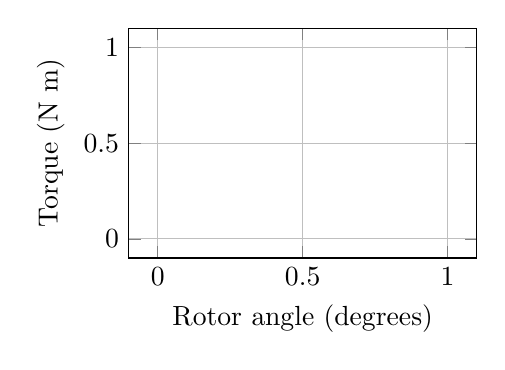
\begin{tikzpicture}
  \begin{axis}[width=6cm,height=4.5cm,
    xlabel={Rotor angle (degrees)},
    ylabel={Torque (N m)},grid=major]
    \femmstudyplot[study=reference-sweep,
      plot options={blue!65!black,mark=*}]
  \end{axis}
\end{tikzpicture}
\end{codeexample}

Every point is a separate equilibrium at the template's currents and frequency.
Positive angles and torque are counterclockwise. Harmonic templates report
cycle-average torque. The curve contains all requested points in their declared
order, including repeated angles; it is not sorted or interpolated by the solver.
A study is registered only after every solve and measurement succeeds.

\begin{command}{\femmanglestudy\opt{\oarg{options}}}
  Compute and register an angular study. Keys belong to |/femm/angle study|.
  Named templates and completed studies have document lifetime. The command
  does not change the current picture's model or draw a figure.
\end{command}
\begin{key}{/femm/angle study/name=\meta{name} (initially empty)}
  Required, unique name of the completed numeric result. Reusing a name fails.
\end{key}
\begin{key}{/femm/angle study/template=\meta{name} (initially empty)}
  Required name of a previously captured sliding band. Geometry, sources,
  frequency and solver tolerances come from that template.
\end{key}
\begin{key}{/femm/angle study/angles=\meta{list} (initially \{0,15,...,90\})}
  PGF foreach list of 1--721 finite angles in degrees. Arithmetic expressions
  are evaluated by PGF. For example, |angles={-30,-15,0,15,30}| examines both
  directions. All angles are relative to the original captured rotor.
\end{key}
\begin{key}{/femm/angle study/quantity=\meta{force, circuit or integrals} (initially force)}
  |force| measures the whole rotor with |method=band|. |circuit| measures a
  named terminal. |integrals| measures the complete domain. Select a compatible
  component when plotting: |torque|, |linkage| for a DC circuit, or |energy|,
  for example. Harmonic circuits use |linkage_real| and |linkage_imaginary|.
\end{key}
\begin{key}{/femm/angle study/circuit=\meta{name} (initially empty)}
  Required for |quantity=circuit|. The circuit must belong to the template;
  its closed signed-turn winding is needed for gauge-independent linkage.
\end{key}
\begin{key}{/femm/angle study/cache prefix=\meta{filename prefix} (initially empty)}
  Empty disables persistent study caches. Otherwise solve $j$ uses
  \meta{prefix}|-j-cache.lfc|, with one-based $j$. Relative names follow the
  TeX output directory. Physical signatures prevent reuse at a changed angle.
  A prefix such as |rotor-study| avoids repeating the solves on the next run.
\end{key}
\begin{key}{/femm/angle study/cache mode=\meta{auto, off, refresh or frozen} (initially auto)}
  Same policy as |/femm/cache/mode|. |frozen| requires a nonempty prefix and
  valid existing caches. Modes and prefixes are local command options; the
  saved numeric study remains available after the surrounding TeX group ends.
\end{key}
\begin{command}{\femmstudyplot\opt{\oarg{options}}}
  Within a PGFPlots axis, issue one ordinary |\addplot+| from a saved angular
  study. This performs no magnetic solve. Keys use |/femm/study plot|.
\end{command}
\begin{key}{/femm/study plot/study=\meta{name} (initially empty)}
  Required completed angle study. Unknown names fail.
\end{key}
\begin{key}{/femm/study plot/component=\meta{component} (initially torque)}
  Finite numeric observable available at every point. The horizontal coordinate
  is always the physical angle in degrees. An unavailable component raises an
  error instead of inserting a zero or omitting a point.
\end{key}
\begin{key}{/femm/study plot/plot options=\meta{PGFPlots options} (initially empty)}
  Passed unchanged to |\addplot+|. Axis limits, tick labels, unit scaling,
  colours, markers and legends remain ordinary PGFPlots choices.
\end{key}
\begin{command}{\femmstudyvalue\marg{study}\marg{index}\marg{component}}
  Expand to one SI numeric result. The index is a one-based integer, not an
  angle. |angle| and |index| are also available numeric components.
\end{command}

\subsection{Differential linkage and impedance matrices}

A matrix uses one common DC bias and its exact mesh. Each column excites one
circuit with a one-ampere, zero-phase incremental current; other independent
sources are zero. The row identifies the observed circuit. No symmetry is
imposed on the computed matrix. With multiple closed windings this gives
self and mutual differential inductances, not secant inductances at the bias.

\begin{codeexample}[width=6cm]
\femmresponsematrix[name=reference-matrix,
  operating point=reference-bias,
  circuits={drive},frequency=50]
\pgfmathprintnumber[sci,precision=3]{%
  \femmmatrixentry{reference-matrix}
    {drive}{drive}{linkage_real}}\,H
\end{codeexample}

\begin{command}{\femmresponsematrix\opt{\oarg{options}}}
  Register a response matrix. Keys belong to |/femm/response matrix|. This
  command preserves the current picture and publishes no partial matrix on
  failure. It always uses incremental permeability; frozen reconstruction is
  a different operation and is not used to define this differential matrix.
\end{command}
\begin{key}{/femm/response matrix/name=\meta{name} (initially empty)}
  Required name, unique among both matrix and angle studies.
\end{key}
\begin{key}{/femm/response matrix/operating point=\meta{name} (initially empty)}
  Required previously captured DC bias. Planar and axisymmetric biases retain
  their ordinary response restrictions; analytical gaps are planar only.
\end{key}
\begin{key}{/femm/response matrix/circuits=\meta{list} (initially empty)}
  Required ordered list of 1--32 distinct existing circuit names. Both row and
  column order follow this list. Circuits must use prescribed series currents
  and closed signed-turn windings. For instance, |circuits={primary,secondary}|
  produces four coefficients from two incremental solves.
\end{key}
\begin{key}{/femm/response matrix/frequency=\meta{frequency} (initially 0)}
  Nonnegative Hz. Zero gives the static differential linkage matrix. Positive
  values give complex linkage and terminal impedance with the peak
  $\exp(+i\omega t)$ convention. Bias phases are not inherited.
\end{key}
\begin{key}{/femm/response matrix/cache prefix=\meta{filename prefix} (initially empty)}
  Same naming and output-directory rules as the angle-study prefix, with the
  column number as index. Use a distinct prefix for each study.
\end{key}
\begin{key}{/femm/response matrix/cache mode=\meta{auto, off, refresh or frozen} (initially auto)}
  Same cache policy and nonempty-prefix requirement for |frozen| as angle
  studies. The default empty prefix keeps the calculation in memory only.
\end{key}
\begin{command}{\femmmatrixentry\marg{matrix}\marg{row circuit}\marg{column circuit}\marg{component}}
  Expand to an SI numeric coefficient. Components are |linkage_real| and
  |linkage_imaginary| in H, and, at positive frequency, |impedance_real| and
  |impedance_imaginary| in $\Omega$ when the terminal voltage is available.
  Imaginary linkage is zero in statics. Closed nonconducting windings can
  provide linkage without a resistive terminal model; unavailable voltage
  components fail explicitly. The output can feed ordinary PGFPlots tables,
  matrix plots or PGF number printing.
\end{command}

\subsection{Rotational sectors}
\begin{key}{/femm/pair/sectors=\meta{integer} (initially 0)}
  Zero retains general rigid pairing. An integer $N\geq2$ sets a rotation of
  $360/N$ degrees from |first| to |second| about the declared |center x| and
  |center y|. It replaces |rotation| and requires zero shifts. A nonzero
  |rotation| or shift is rejected. Antiperiodic pairing requires even $N$ so
  that a complete revolution restores the sign. Material and source symmetry
  remain the user's physical assumption, not a conclusion of mesh pairing.
\end{key}

The following half-domain has $A_z=x\,\mathrm{T}$, hence a uniform downward
field. Its two radial cuts are antiperiodic images. Pairing synchronises their
mesh nodes before reducing the signed degrees of freedom. The same interface
also works for supported fixed-frequency harmonic sectors.

\begin{codeexample}[width=5cm]
\begin{tikzpicture}[scale=2,
 femm/problem={xmin=-10,xmax=10,
   ymin=0,ymax=10,mesh size=2,depth=5},
 femm/pair={first=a,second=b,
   sectors=2,type=antiperiodic}]
 \path[femm/domain] (-10,0) rectangle (10,10);
 \draw[femm/frontier={name=a,type=periodic}]
   (0,0)--(10,0);
 \draw[femm/frontier={name=b,type=periodic}]
   (0,0)--(-10,0);
 \draw[femm/frontier={name=outer,x coefficient=1}]
   (10,0)--(10,10)--(-10,10)--(-10,0);
 \pic[femm/lines=9] {femm field};
\end{tikzpicture}
\end{codeexample}

Sector integrals, forces and winding linkage refer to the declared sector.
They are not automatically multiplied by $N$. Decide which whole-machine
quantity is wanted before applying a symmetry factor. Reduced-sector analytical sliding uses separate body reference frames;
see Section~\ref{sec:sector-gaps}. That chapter also describes passive native
AGE record preservation. Native AGE field import is described in
Section~\ref{sec:native-gaps}; eccentric P1 positions in Section~\ref{sec:eccentric}.

\subsection{Analytical operator, observables and convergence}
Let $t=\log(r/r_i)$ and $L=\log(r_o/r_i)$. Angular P1 trace functions are
projected by exact integration onto a mean and sine/cosine modes. For each
positive order $n$, the inner and outer coefficients $a_i,a_o$ determine
\[
 a(t)=a_i\frac{\sinh(n(L-t))}{\sinh(nL)}
       +a_o\frac{\sinh(nt)}{\sinh(nL)}.
\]
The mean is linear in $t$. Its weak matrix is
$2\pi L^{-1}\bigl(\begin{smallmatrix}1&-1\\-1&1\end{smallmatrix}\bigr)$;
each sine or cosine mode contributes
\[
 \pi n\begin{pmatrix}\coth(nL)&-\operatorname{csch}(nL)\\
       -\operatorname{csch}(nL)&\coth(nL)\end{pmatrix}.
\]
Trace projection lifts this symmetric operator to the bulk nodal potentials.
The constant null mode is preserved. Trace vertices are projected to the exact
circles after meshing; bulk triangles are audited again for positive area,
coverage and conformity. Keep the required empty collar on both sides.

Point sampling and profiles inside the physical annulus use the analytical
curl, including both phasor parts. |method=band| integrates Maxwell traction
on the geometric-mean-radius circle. Angular quadrature resolves every product
of retained modes; first mechanical variations use the captured bias field.
Whole-gap energy uses the same modal quadratic form as the solve, with the
usual one-half factor for cycle-averaged peak phasors. A regional energy
selection must contain all visual gap triangles or none of them: modal energy
cannot be assigned independently to individual display triangles.

Field-line display still contours the nodal potential on the visual band
triangulation. Thus the displayed curves approximate the analytical field;
increasing angular segmentation improves that drawing. Regional field averages
retain their ordinary triangle quadrature. A small linear residual does not
bound bulk, trace-projection or Fourier truncation error. Check convergence of
torque, linkage and energy separately. The tests include exact annular modes,
constant-potential invariance, the fixed-current coenergy derivative and
unchanged-field cache restoration. Native P1 response exchange is described
in Section~\ref{sec:response-exchange}.
